% --- Theoretical Foundations ---
\begin{frame}{Why Does SSL Work?}
  \begin{itemize}\itemsep0.28em
    \item Exploits \textbf{structure} in natural data (spatial context, temporal continuity, language statistics).
    \item Contrastive methods stress \textbf{invariances} to augmentations; reconstruction methods force \textbf{complete} explanations of the input; JEPA emphasizes \textbf{predictive} structure in \textbf{representation space}.
    \item Strong \textbf{linear / low-data probes} suggest encoders expose semantically useful axes for downstream tasks.
    \item Active research: theoretical limits, failure modes (shortcuts), and unified views across the three families above.
  \end{itemize}
\end{frame}

% --- I-JEPA: Three SSL paradigms (Meta blog) ---
\begin{frame}{SSL Paradigms: Invariant, Generative, and Predictive (JEPA)}
    \begin{itemize}\footnotesize
      \item \textbf{(a) Joint-embedding (invariance):} map views $x,y$ to embeddings and pull compatible pairs together---can bias toward invariance shortcuts.
      \item \textbf{(b) Generative:} decode $\hat{y}$ from context $x$ (and latent $z$), loss in \textbf{pixel/input space}---must explain unpredictable detail.
      \item \textbf{(c) JEPA:} predict \textbf{embedding} $\hat{s}_y$ of $y$ from context; compare to $s_y$ from a target encoder---semantic, discard irrelevant variability.
    \end{itemize}
    \centering
    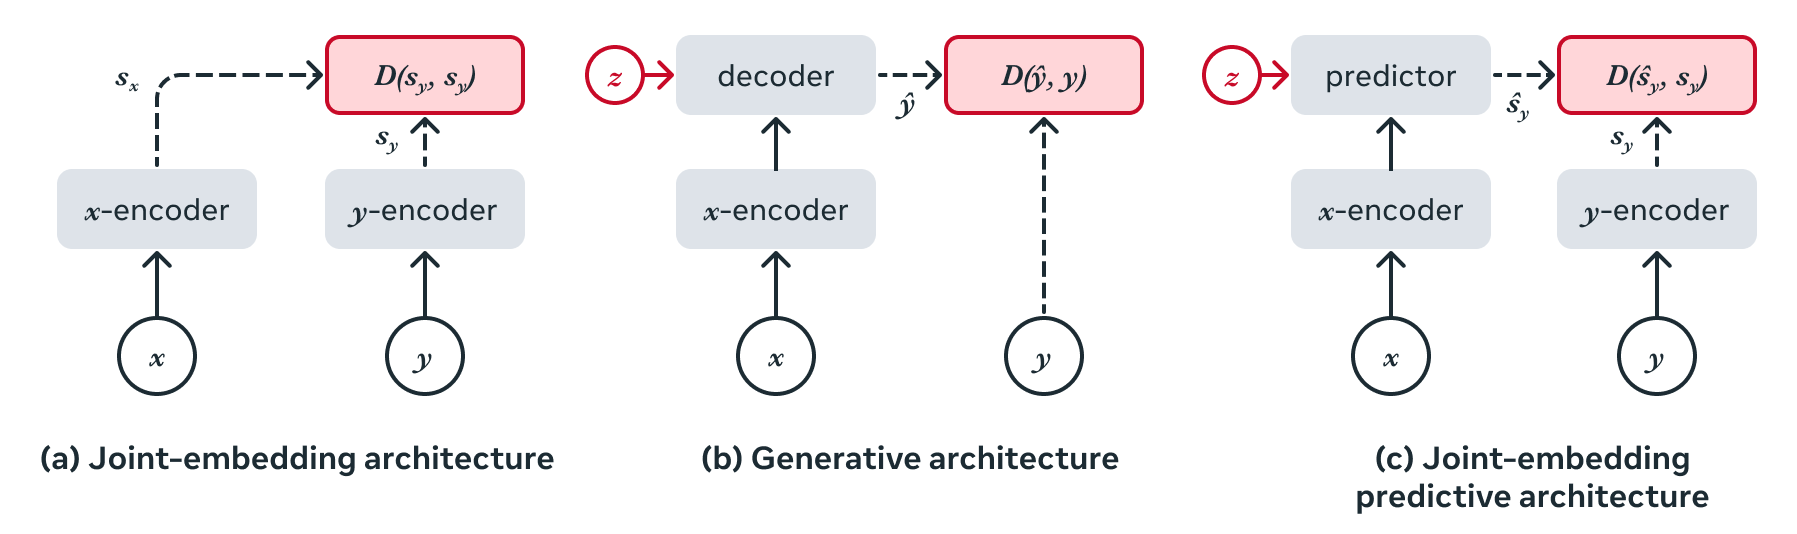
\includegraphics[width=0.8\linewidth, height=0.6\textheight, keepaspectratio]{assets/New-Lecture_JEPA_models/ijepa_blog_ssl_paradigms.png}
    \linebreak
    {\scriptsize Reference: Adapted from Meta I-JEPA blog.}
\end{frame}
